\documentclass[10pt, compress, handout]{beamer}

\usetheme{utopia}

\usepackage{booktabs}
\usepackage[scale=2]{ccicons}
\usepackage[outputdir=out]{minted}
\usepackage{natbib}

\usepgfplotslibrary{dateplot}

\usetikzlibrary{shapes,arrows,positioning,intersections}
\tikzstyle{block} = [rectangle, draw, fill=blue!20,
    text width=5em, text centered, rounded corners, minimum height=4em]
\tikzstyle{line} = [draw, -latex']


\usemintedstyle{trac}

\hypersetup{colorlinks=false}

\title{Machine Learning in Systems Biology I\\(Unsupervised)}
\subtitle{}
\date{29.06.2022}
\author{Jonas Pleyer}
\institute{Freiburg Center for Data Analysis and Modeling (FDM)}

\begin{document}

\maketitle

\section{Introduction}
\label{sec:introduction}
\subsection{What is Machine Learning?}
\label{subsec:introduction-definition}
\begin{frame}{\insertsubsection}
    'A computer program is said to learn from experience $E$ with respect to some class of tasks $T$ and performance measure $P$ if its performance at tasks in $T$, as measured by $P$, improves with experience $E$'\\
    - Tom M. Mitchell~\cite{Mitchell1997}
\end{frame}
%
%
\subsection{History of Machine Learning}
\label{subsec:introduction-history}
\begin{frame}{\insertsubsection}
    \begin{itemize}[<+->]
        \item[1943] First publication of neural network~\cite{McCulloch1943}
        \item[1956] Dartmouth Summer Research Project (Birthplace of modern Machine Learning)
        \item[1965] Nilson Machine Learning for pattern classification~\cite{Nilsson1965}
        \item[1966] Following years: Many setbacks in Artificial Intelligence called 'AI-Winters'
        \item[1995] Support Vector Machines are first introduced
        \item[2002] Torch first release (open source library)
        \item[2006] Geoffrey Hinton coins 'Deep Learning'~\cite{Hinton2006}
        \item[>2006] Companies such as Netflix, Facebook, Microsoft, Google fund projects/prizes in and use machine learning/artificial intelligence
    \end{itemize}
\end{frame}
%
%
\subsection{Workflow}
\label{subsec:introduction-workflow}
\begin{frame}{\insertsubsection}
    Machine learning techniques follow a similar workflow.
    \begin{enumerate}[<+->]
        \item Define Problem (scope, feasability)
        \item Gather Data (assumptions, constraints)
        \item Pre-process Data (cleanup, drop)
        \item Analyze Data (define features, find correlations)
        \item Prepare Data (transform, normalize, drop)
        \item Evaluate Models (train/test, classify/regress)
        \item Tune Model (cross validation, fine tune parameters)
        \item Apply model to problems, learn more
    \end{enumerate}
\end{frame}
\section{Concepts}
\label{sec:concepts}
\subsection{Unsupervised and Supervised Learning}
\label{subsec:concepts-un-supervised-learning}
\begin{frame}{\insertsubsection}
    Supervised
    \pause
    \begin{itemize}[<+->]
        \item Fit model to labelled data (ie. with 'ground truth')
        \item Data is usually obtained experimentally or assigned by humans
        \item Previously labelled data can serve as testing set
    \end{itemize}
    \pause
    Unsupvervised
    \pause
    \begin{itemize}[<+->]
        \item Data does not contain any labels (only inputs)
        \item Find structure in data (clustering, grouping)
    \end{itemize}
    \pause
    Semi-supervised
    \pause
    \begin{itemize}[<+->]
        \item Combine partly labeled data with partly unlabeled data
        \item Can have huge performance benefits compared to unsupervised learning
    \end{itemize}
    This section follows~\cite{Greener2021}.
\end{frame}
%
%
\subsection{Terms}
\label{subsec:concepts-terms}
\begin{frame}{\insertsubsection}
    \pause
    \begin{itemize}[<+->]
        \item Classification: Assign datapoints discrete categories (eg. cancerous, non-cancerous). Algorithms are called 'classifiers'.
        \item[] If discrete categories are mutually exclusive, we call them 'classes', otherwise 'labels'.
        \item Regression: Output continuous values (eg. predict free energy of protein system).
        \item Classification problems can also be solved with regression and thresholds/binning.
        \item Clustering: Predict groupings of similar datapoints.
    \end{itemize}
\end{frame}
%
%
\begin{frame}{\insertsubsection}
    \begin{itemize}[<+->]
        \item Loss or Cost function:\\
        Measure deviation to ground truth in supervised learning.
        Implemented similarly in unsupervised situations.
        \item Parameters: Part of the model, will be adjusted by learning process of the model.
        \item Hyperparameters: Not part of the model but control learning process (eg. learning rate, number of iterations)
        \item Training: describes process of iterative learning and adjusting the parameters of the model to obtain better performance. Minimize the loss/cost-function.
        \item Validation: Use seperate dataset to test model.
    \end{itemize}
\end{frame}
%
%
\begin{frame}{\insertsubsection}
    \begin{figure}
        \centering
        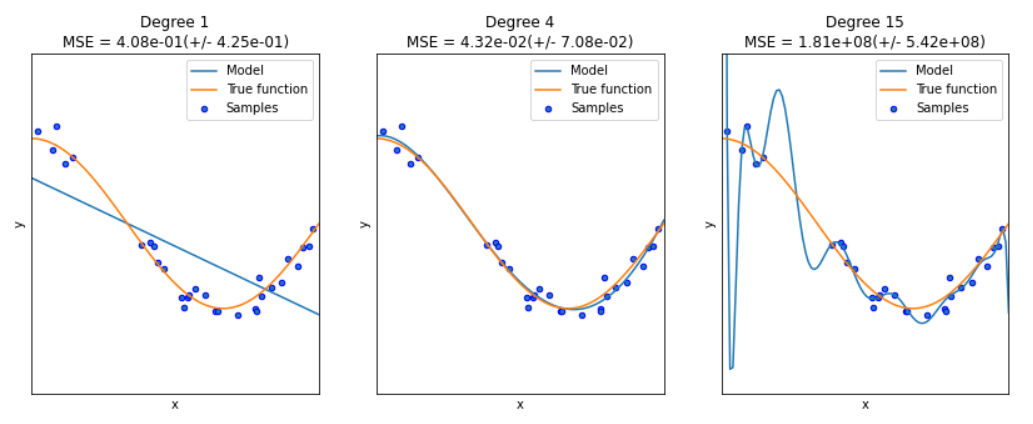
\includegraphics[width=\textwidth]{media/underfitting_and_overfitting_in_machine_learning_image.png}
        \caption{Underfitting, Optimal Fitting and Overfitting~\cite{Tripathi2020}}
    \end{figure}
\end{frame}
%
%
\subsection{Inductive Bias and Variance}
\label{subsec:concepts-bias-variance}
\begin{frame}{\insertsubsection}
    \begin{itemize}[<+->]
        \item Inductive Bias: Set of assumptions.
        \item[] Leads it to favour a particular type of solution over others.
        \item[] Often programmed in mathematical model.
        \item[] Example: Recurrent Neural Networks anticipate sequential dependencies
        \item Trade-off between bias and variance
        \item[] Different inductive biases typically lead to better performance, but higher constraints on the model.
        \item[] Lower bias makes fewer assumptions.
        \item Variance: How much does trained model change in response to training on different dataset.
        \item We want low bias and low variance.
        \item Low bias and low variance often conflict each other.
        \item[]$\Rightarrow$ Need to balance between them
    \end{itemize}
\end{frame}
\section{Machine Learning Techniques}
\label{sec:ml-techniques}
\subsection{Traditional Machine Learning Techniques}
\label{subsec:concepts-traditional-techniques}
\begin{frame}{\insertsubsection}
    \begin{figure}
        \centering
        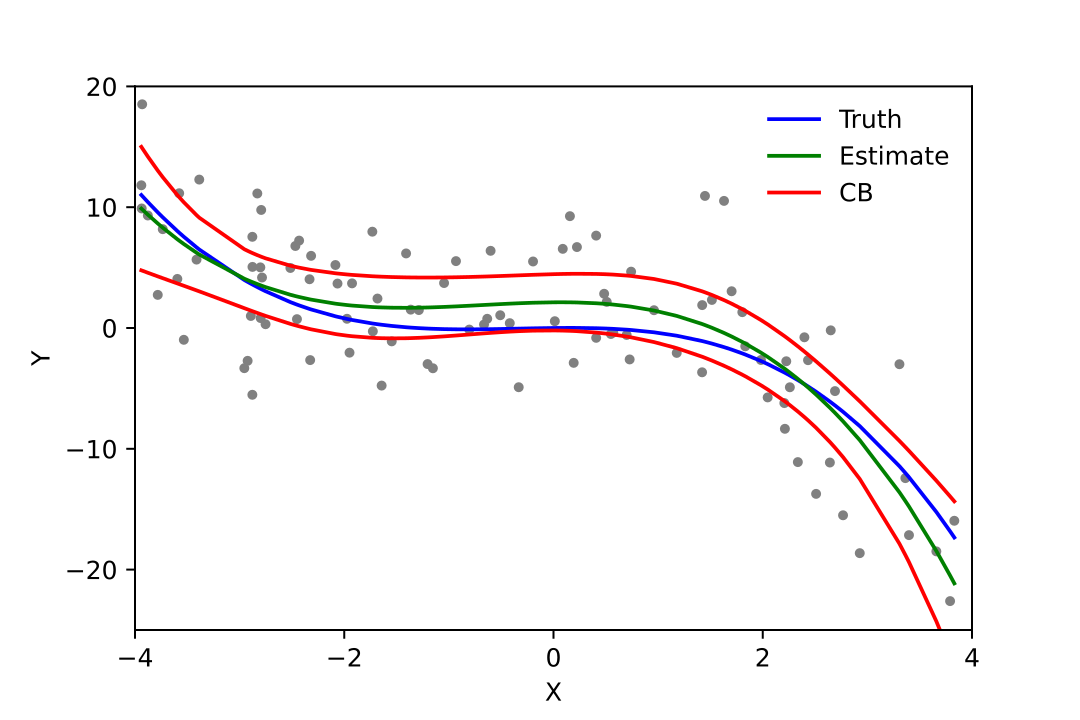
\includegraphics[width=0.8\textwidth]{media/Polyreg_scheffe.png}
        \caption{Polynomial Regression~\cite{Skbkekas2009}}
    \end{figure}
\end{frame}
%
%
\begin{frame}{\insertsubsection}
    \begin{figure}
        \centering
        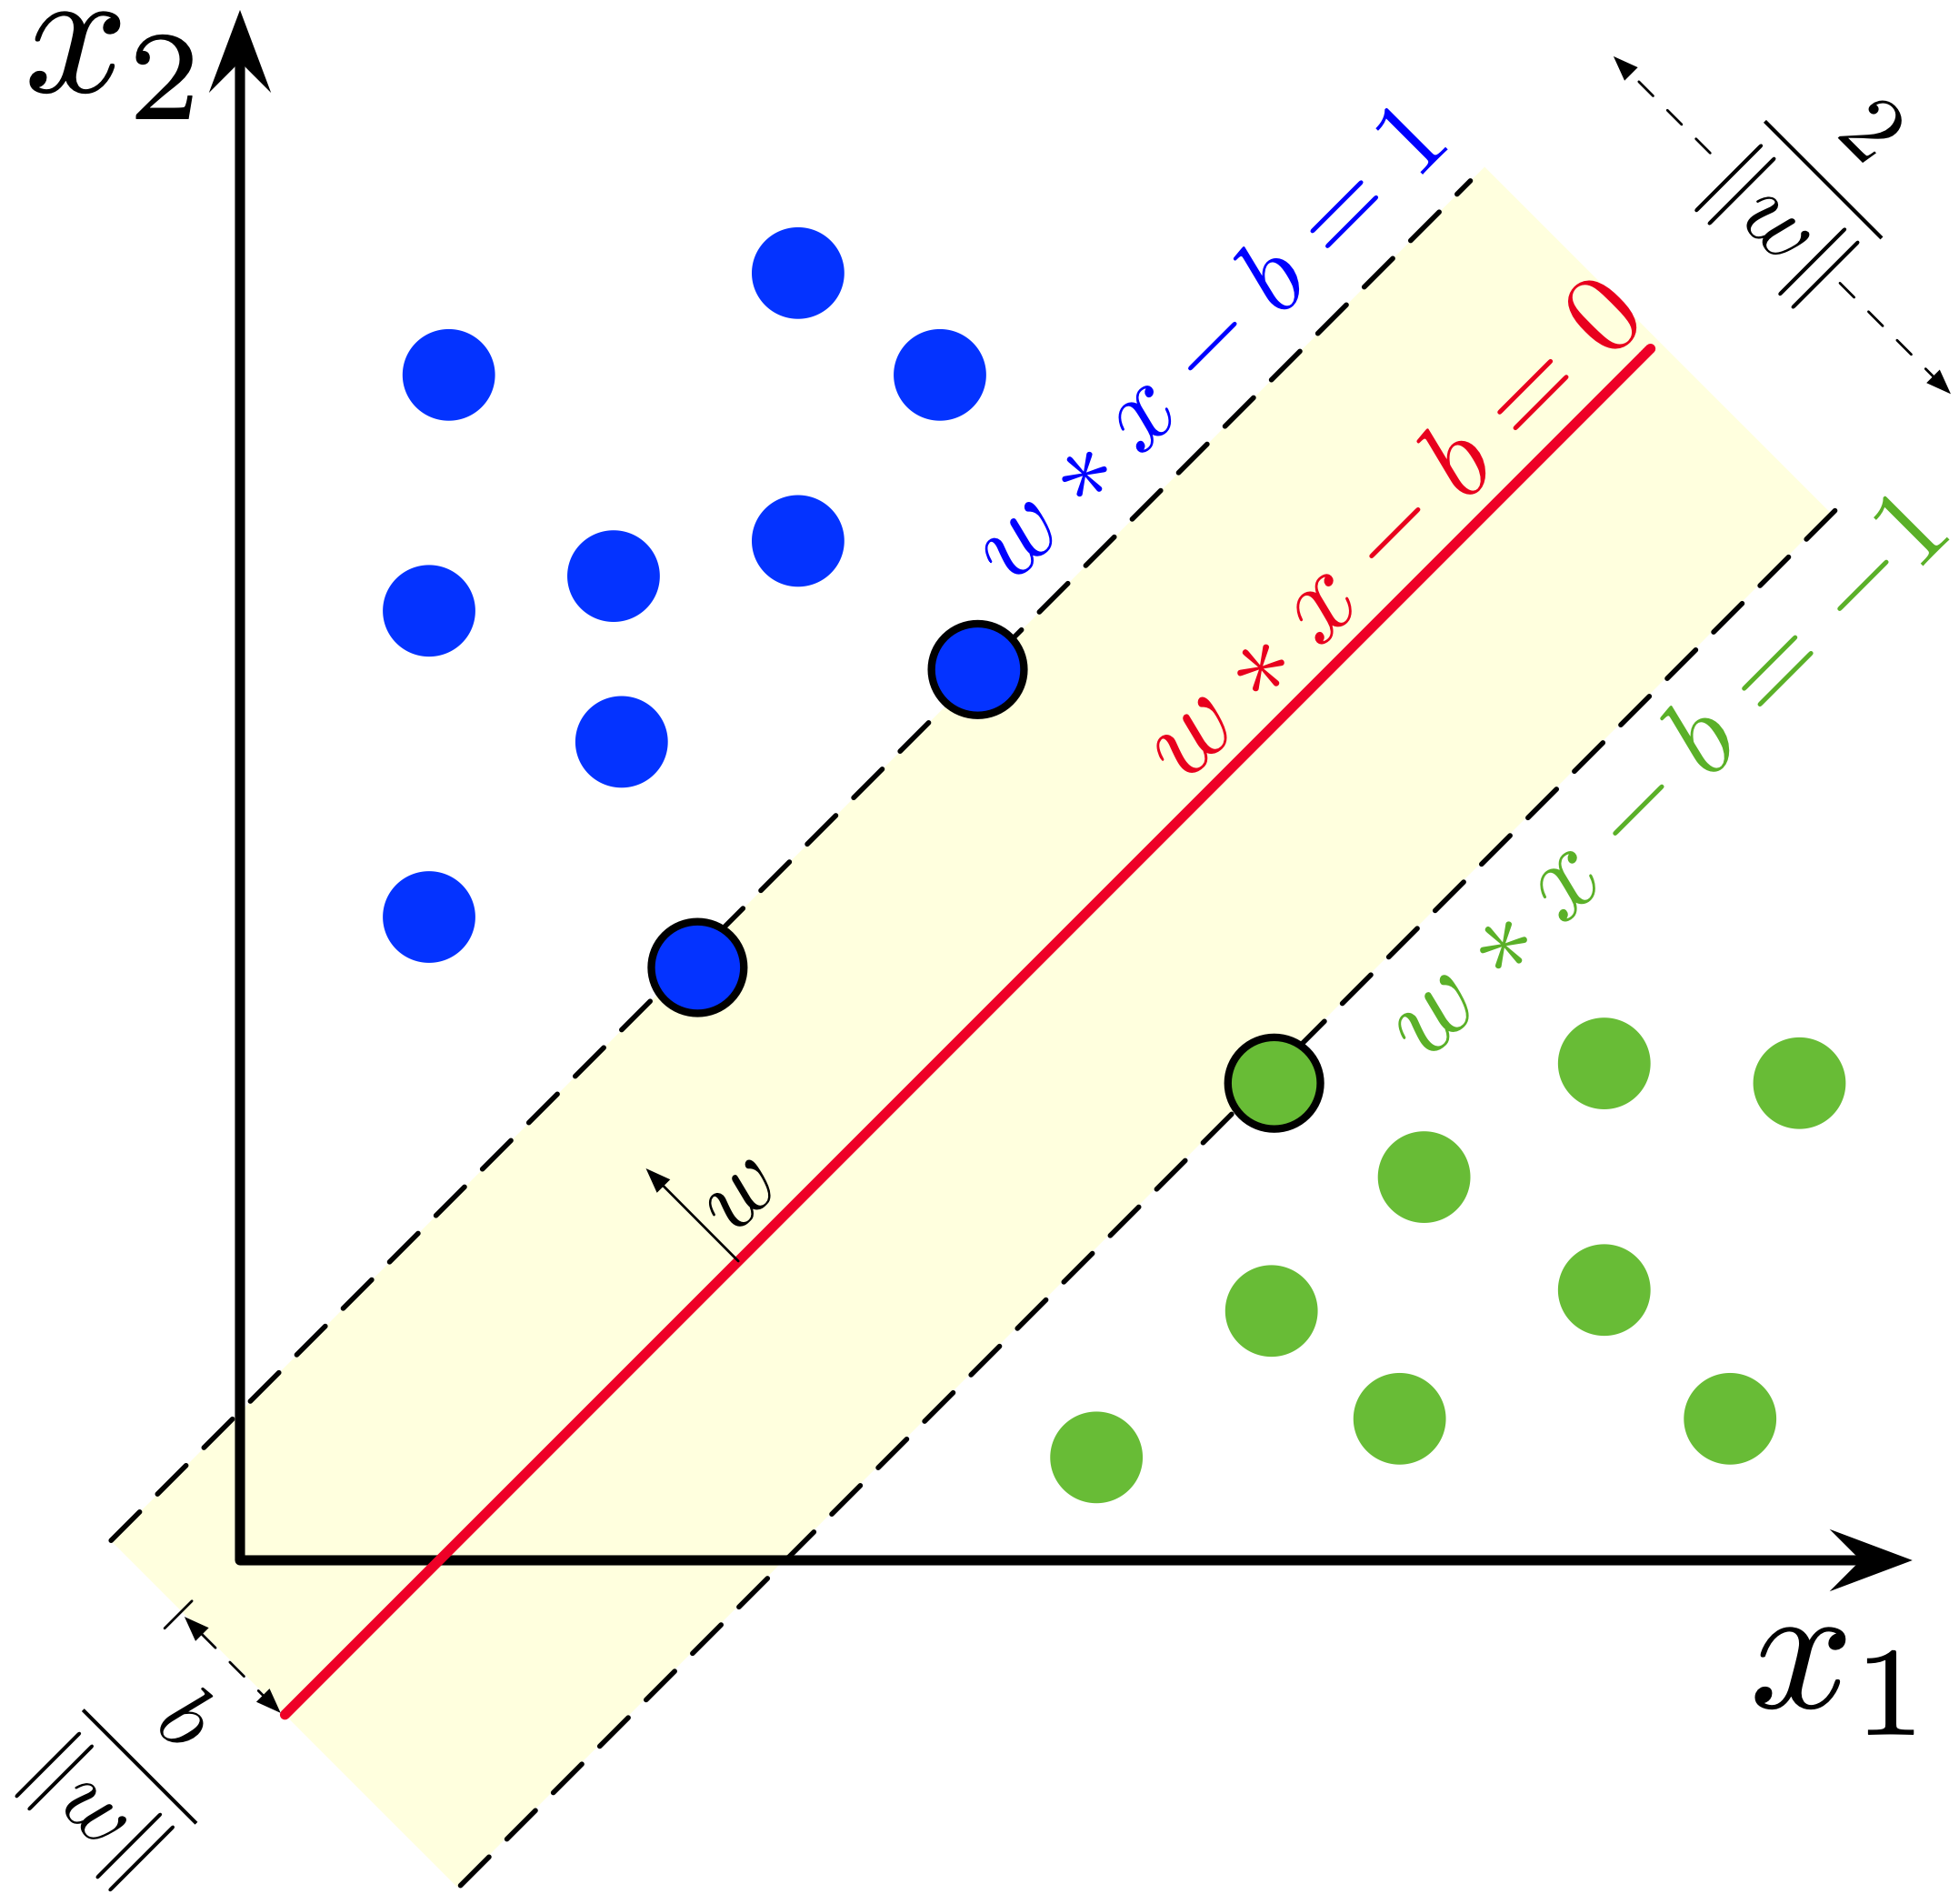
\includegraphics[width=0.6\textwidth]{media/SVM_margin.png}
        \caption{Support Vector Machine~\cite{Larhmam2018}}
    \end{figure}
\end{frame}
%
%
\begin{frame}{\insertsubsection}
    \begin{itemize}
        \item Traditional machine learning routines should be preferred over neural networks
        \item Deep learning can be powerful (and trendy)
        \item[] However, currently still limited in applicability
        \item[] Requires lots of data $\Rightarrow$ often not present
        \item Traditional Methods are faster to develop and test
        \item[] They typically expect same number of features with each datapoint
        \item[] $\Rightarrow$ Padding and Windowing are methods to circumvent this
    \end{itemize}
\end{frame}
%
%

\section{Biology again}
\label{sec:biology-again}
\begin{frame}{\insertsubsection}
    
\end{frame}

\plain{Questions?}

\begin{frame}{Literature}
    \bibliographystyle{alpha}
    \bibliography{literature}
\end{frame}
% 
%
\end{document}
